\documentclass[11pt, a4paper]{article}

% \usepackage{titlesec}

% \titlespacing*{\section}
% {0pt}{7ex}{7ex}

%%%%%%%%%
%% Packages
%%%%%%%%%

% Font encoding
\usepackage[utf8]{inputenc}
\usepackage[T1]{fontenc}
\usepackage[english]{babel}
\usepackage{csquotes}
\usepackage{url}
\usepackage{color}
\usepackage{listings}
\usepackage{listings-golang}
% \usepackage[square,sort,comma,numbers]{natbib}
% \bibliographystyle{plain}

% Used for including graphics
\usepackage{graphicx}

%\usepackage[numbers]{natbib}
% \usepackage[defernumbers=true]{biblatex}
%\usepackage[sort,nocompress]{cite}

\usepackage{enumitem}

\usepackage{filecontents}


%%%%%%
%% Layout
%%%%%%

\setlength{\oddsidemargin}{0pt}
\setlength{\topmargin}{0pt}
\setlength{\textheight}{600pt}
\setlength{\textwidth}{460pt}
\setlength{\headsep}{10pt}
\setlength{\parindent}{0cm}

% Avoid line breaks
\sloppy

% code snippets
\lstset{
  language=Golang,
  aboveskip=3mm,
  belowskip=3mm,
  showstringspaces=false,
  columns=flexible,
  basicstyle={\small\ttfamily},
  numbers=none,
  numberstyle=\tiny\color{gray},
  keywordstyle=\color{blue},
  commentstyle=\color{dkgreen},
  stringstyle=\color{mauve},
  breaklines=true,
  breakatwhitespace=true,
  tabsize=3
}


%%%%%%
%% Data
%%%%%%

\newcommand{\authors}{Julien Perrenoud, Loïc Serafin, Guillaume Vizier}
\renewcommand{\title}{A Secure Peerster}

\begin{document}

\begin{titlepage}
	\centering
	
\includegraphics[scale=0.1]{epfl.png} \par
	\vspace{1.5cm}

	{\scshape\Large Decentralized Systems Engineering Project\par}
	\vspace{1.5cm}
	{\huge\bfseries \title \par}
	\vspace{2cm}
	{\Large\itshape \authors \par}
	\vfill
	\vfill

    % Bottom of the page
	{\large \today \par}

\end{titlepage}

\tableofcontents

\newpage

\section{Introduction}

    % We plan to add an anonymity and trust component to one of our current implementations of the Peerster.
    The initial implementation of Peerster contains several security flaws that a malicious node could exploit.
    First of all, the private messages are sent through the network in plain text.
    Therefore, it is very easy for any node on the direct path of a private message to intercept such messages and listen to the private conversation between two peers.
    Secondly, any node is able to register and announce any possible name to the network.
    Such a name is then used as is by other nodes, without checking if the node actually exists and there is no check for uses of the same name by different nodes, which leaves open the possibility of spoofing anyone on the network.
    Finally, the traffic from a node is relayed immediately by the neighbors, in a way that everybody is aware of the original sender of a message.
    % Finally, there is no anonymity for the sender of a message. As the messages are relayed directly by the
    % This means that it is not possible to be anonymous on the network.
    In this project, we aim to fix some of these flaws and overall increase the level of anonymity and privacy of users on Peerster.
    First, we will implement privacy of content via public key cryptography.
    Second, a basic mix network routing algorithm will be implemented to guarantee sender anonymity.
    Finally, we will use the already existing blockchain as a decentralized directory of public keys and mixer nodes.

    % Secondly, the private messages are sent in plain text.


    % Indeed, at the time of this writing, we can spoof the name of any gossiper (existing or not), and every message can be intercepted, modified, duplicated, ...
    % As the Peerster is a tool for a community, and provided that this community is constituted of human beings, we can rightfully expect a certain level of maliciousness.
    % Thus, we plan to cypher and sign every message send through our gossipers, by using an asymmetric encryption scheme.
    % Public keys will be shared through the blockchain. We also plan to anonymize the routing of the messages in the gossiping protocol.

\section{Related work}

    \subsection{Signature and encryption}

        Two main schemes exist for cyphering/decyphering messages, and for signing/verifying the signature: using a symmetric cryptographic scheme, or an asymmetric one.
        \bigbreak
        Symmetric cryptographic schemes use the same key on both participants to the exchange of messages.
        The issue in our case is that we would need to create one key for each pair of peers in our network, leading to a combinatory explosion of the number of keys.
        In addition, two nodes would need to exchange their common key through a secure channel, which can only be created \textbf{after} they agreed on a key to use.
        \bigbreak
        Asymmetric schemes make each user create a \textbf{pair} of keys: a public key and a private key.
        The public key is for public usage: its purpose is to be shared with everybody on the network (and beyond).
        The private key has to be kept secret by its owner.
        In this case, a node signs a message using its private key, and every node having the public key can verify the signature.
        To cypher a message, a node uses the public key of the destination, and only the private key can reverse the operation.
        \bigbreak
        One issue remains: the transmission of the keys.
        Using an asymmetric encryption scheme, we do not bother with exchanging the keys in a secure way, because only the public key, which is common knowledge, is sent.
        However, the mapping $gossiper~name \rightarrow public~key$ is still problematic.
        Indeed, as of today, any node can transmit any received public key as belonging to it, in the context of a man in the middle attack.
        \bigbreak
        In the web of trust, it is advised to physically meet the person we are exchanging keys with.
        In our setting, we will propose a transaction containing a public key, along with the name of the owner and this name signed with the private key corresponding to the public key.
        Signing one's public key before sending it on a keys server is a practice advised for distributed systems of trust.

    \subsection{Mix Networks}

        Mix networks are a class of anonymous and hard-to-trace routing protocols initially described by David Chaum in the 1981 paper \textit{Untraceable Electronic Mail, Return Addresses, and Digital Pseudonyms} \cite{chaum84}.
        These protocols aim at implementing \textbf{forward anonymity} (i.e. concealing the identity of the sender of a message) by routing the message through a series of relay (or "mixer") nodes.
        % A mixer node will then typically wait until a certain number of messages has been reached before shuffling and forwarding the messages in random order to the next relay.
        Each such node will remove information about the origin of the message and place it in a queue.
        Once a specific condition is met, the mixer node will shuffle the queue and forward the messages in a different order to the next relay.
        Finally, it is important to note that before a message is sent on a mixnet, it needs to be encrypted behind several layers of security (one for each mixer node on the path, who will decrypt it one layer at a time).
        Besides the obvious task of making the input of a shuffle indistinguishable from its output, this multi-layer encryption-decryption scheme (often called an \textit{Onion}) ensures that a given message will follow its intended path and that the mixer nodes cannot read its content
        % Finally, in order to ensure that mixer nodes cannot themselves access the content of the messages,
        % There are many ways
        \bigbreak
        In practice, mix networks were and are still often used as a way to anonymously browse the web or communicate via e-mail.
        This second kind is often distinguished in three\footnote{This does not consider type 0 remailers comprised of a single node, as it is less relevant here.} types. \
        \textbf{Type I} (or \textit{Cypherpunk}) remailers provide a simple implementation of Chaum's mix network.
        However, the implementation contained several security flaws.
        Mainly, the length of the original message was kept the same, and the messages were always forwarded with a fixed delay (if any).
        This made it possible to track the path of a given message through the network by looking at the lengths and timings of the messages exchanged between the mix nodes.
        % which made it possible to track a message by looking at the length of packets exchanged between multiple nodes.
        % Secondly, type I remailers usually forwarded messages with a fixed delay (if any), which allowed one to track a message by looking at the timing.
        These issues were addressed in 1995 by Lance Cottrell who released \textit{MixMaster}, an implementation now referred to as a \textbf{type II} remailer.
        Finally in 2002, a \textbf{type III} remailer known as \textit{MixMinion} \cite{mixminion} further improved on MixMaster.
        Amongst other things, MixMinion allows users to specify single use reply blocks that enable the recipient to anonymously respond to an incoming message.

        % Such issues were addressed by Lance Cottrell in his 1995

        % This original remailer was improved upon by Lance Cottrell in his 1995 implementation named \textit{MixMaster}.
        % It has several security flaws however,  \textbf{Type II} remailers such as \textit{Mixmaster} try to fix some of the flaws, namely hiding  \textbf{type III} bla bla
        % Anonymous
        % Further work such as \textit{MixMinion} further improved the original models by providing

        % There are many examples of successful mix networks

        % wait until a certain number of messages has been reached before shuffling and forwarding the messages in random order to the next relay.
        % Each mixer node will remove any information about the origin of the message and store it in a queue of a given size.
        % that remove any information with the origin of the message,


        % In order to do this, mix networks create
        % were first originated by David Chaum in.
        % The main idea of mix network is to  conceal the identify of the sender sender anonymity by creating a path through a series of relay (or "mixer") nodes.
        % These nodes typically wait until a certain number of messages has been reached ("threshold node") or a certain time has elapsed ( .. ) before shuffling and forwarding the messages in random order to the next relay.
        % The final relay then
        % We usually distinguish three types of mix networks: \textbf{type I} bla ba bla , \textbf{type II} bla bla, \textbf{type III} bla bla

    % \subsection{Tor}
        \bigbreak
        Lastly, it would be hard to discuss anonymous routing protocols without mentioning \textbf{Tor} (shorthand for \textit{The Onion Router}).
        Initially describe in \cite{tor}, Tor is also derived from Chaum's original mix network and is in some ways very similar to the concepts explained above.
        The main difference is that a Tor relay nodes will simply wait a random delay before forwarding an incoming message, without performing any kind of shuffle.
        The main advantage of this is a big reduction in latency.
        Indeed, classic mixer nodes - who wait for a given number of incoming messages before forwarding them - might end up causing arbitrarily large delays in the delivery of a message.
        On the other hand, there is a clear trade-off with the security of the system, as one can argue that not shuffling messages allows one to trace a particular connection more easily.
        This is fair, however the performance of Tor is based on two key assumptions.
        First, the network should always be fairly busy.
        This will help disguise the traffic as it blends in with requests from other peers.
        Secondly, it is unlikely that someone will get access to the logs of every one of the nodes on the path of a message (which would be required to perform a successful attack on the message).
        % builds its security on top of the fact that it is unlikely
        % this has the effect of lowering the overall performance of the protocol.

        % to wait until they reach a certain number
        % This has the main advantage of

        % Instead, it will simply wait a random delay before forwarding them, relying on a relatively busy traffic.

        \subsection{Mixer Node Location and Storage of Keys}

        % Intro
        Even with a list of public keys and mixer nodes, one still needs to trust these data.
        They might be forged by malicious users in the network and are hardly detectable.

        To ensure the security of communication data in he network, there are several ways to proceed.
        First of all, we can of course give the example of the physical meeting between the different users of the networks as well as those hosting mixer nodes to exchange public keys and mixer nodes addresses.
        But this kind of solution is never used practically speaking for user convenience.
        Another solution is to have a trusted third party that distributes to all users required data.

        %- Type I remailer = third party je crois http://www.noreply.org/echolot/rlist2.html
        In \textit{Cypherpunk} and \textit{Mixmaster} (types I \& II remailers), those third parties are hosted by trusted groups.
        For example, a list of available and trusted remailers can be found at all times on noreply.org\footnote{\url{http://www.noreply.org/echolot/rlist2.html}}

        % mixmion = DHT (https://www.mixminion.net/minion-design.pdf)
        In Mixminion\cite{mixminion}, the third party is a set of directory servers managing a \textit{Distributed Hash Table} (DHT) possibly hosted by the users themselves.
        These directory servers together manage the state of the mixer node network and the keys of all nodes in the system.
        This system generally makes it possible to distribute reliable data, but several attacks remain possible, in particular by exploiting the difference in knowledge of the different directory servers.
        The explanation for the attack is given in Mixminion design\cite{mixminion} paper in section 6.

        %- Compare vs Blockchain


\section{System goals and functionalities and architecture}

    In this section, we will first discuss the goals of the improvements we plan to make on top of our Peerster implementation(s).
    We will then precise the foreseen functionalities to reach these goals, to finally discuss the architecture of our system.

    \subsection{System goals}a\label{subsec:system-goals}
        Our main goal is to improve the security and the anonymity of the Peerster.

        Starting with such an unsafe specification, and given the little time we have to put our ideas in practice, we had to make tough choices.
        Thus we decided to focus on the cyphering and signing of all exchanges, with a mapping $gossiper~name \rightarrow public~key$ stored in the blockchain\footnote{We are aware that the so-called ``blockchain'' is not actually a blockchain, but we have to make concessions here.} for different nodes to know the same peers.

        The second main goal of the project is to anonymize users' message by using the Mix-network system proposed by David Chaum\cite{chaum84}, creating a route of several mixing nodes before reaching a message recipient, and shuffling messages in random order so that it could not be traced back in time.

    \subsection{Functionalities}\label{subsec:functionalities}

        \begin{itemize}

        \item \textbf{Public Key Cryptography} -
        We will add, during the starting process of a node, the creation of a pair (public key, private key), along with the creation of a transaction, broadcast to the network, for the public key to be known by other peers in the network.
        We will still be vulnerable to man-in-the-middle attacks, but if we assume that the public keys are correctly linked to their possessor, as we assume that private keys cannot be forged or stolen, we should be safe against packet modifications and creation.

        \item \textbf{Security} - We will also replace the current calls to \texttt{WriteToUDP} by calls to a function to be implemented, that will cypher and sign a message. Also, we will replace the reception of a message (namely \texttt{ReadFromUDP}) by a call to another function, also to be implemented, that decypher and verify the signature of any received packet.

        \item \textbf{Blockchain-Based Key Directory} -
        It is not enough to create public and private key pairs for the network to be secure.
        Having all gossipers exchange directly their public keys through the Peerster network has many flaws, e.g. a simple man-in-the-middle attack, intercepting public key exchange and giving his own public key to catch all messages from the conversation.
        We plan to reuse our implemented blockchain to store everyone's public key alongside the current filenames mapping. This shared structure will prevent such attacks or at least make them detectable.
        We also need to have a trusted third-party to hold the list of mixing nodes and the list of pseudonyms.

        \item \textbf{Download Chain History} -
        In order to allow nodes joining after the creation, we will modify the current implementation of the blockchain by allowing the creation of a genesis block and the ability for a node to download the entire history of the chain from the previous nodes.
        We propose to build this using the gossip mechanism already in place, using new type of messages that will be exchanged between nodes arriving in the network and those already up to date.

        \item \textbf{Mixer Nodes} -
        Our first step towards the implementation of a mix network will be to upgrade each node to a potential mixer node.
        That means, each node should be capable of receiving, batching, deciphering, shuffling and forwarding messages to another node.
        In order to batch messages properly, mixer nodes will implement a simple threshold policy: waiting until a constant number of messages has been reached and then simply outputting a message at random.

        \item \textbf{Anonymous Routing} -
        Once mixer nodes are in places, we will give the nodes the possibility to conceal all of their communications by routing them through a series of  nodes.
        This will be implemented via a new message type \texttt{OnionPacket} that wraps around a regular \texttt{GossipPacket}.
        When a node receives and deciphers such a packet, it can detect whether the packet is fully decrypted or not.
        If it is, the node will process its content as a regular \texttt{GossipPacket}.
        If it is not, it will forward it to the next node in the chain.

        \item \textbf{Blockchain-Based Mixer Nodes Directory} -
        To plan a routing path through several mixer nodes, one must know in advance multiple mixer nodes addresses.
        As for public keys, we decided to choose the blockchain to store the addresses of all mixer nodes when these mixer nodes manifest as such.

        \end{itemize}

    \subsection{Architecture}

    % Cryptography
    % - Ability to create private/public keys on a node
    % - Publish these keys on the blockchain
    % - New message type "SecurePrivateMessage" (same as private message but encrypted)
    % - Encrypt private messages with keys
    % - Decrypt private messages
    % - Display in GUI

    % Mixnet
    % - Implement core behavior inside a mix node
    %     - Shuffling
    %     - Encryption (using part 1)
    %     - Padding messages
    %     - Batching
    % - Check how it works when one node goes down or a malicious node is present

    % Blockchain
    % - Stores the public keys available on the network
    % - Stores a return address for a public key
    % -
    % - Fixing the blockchain’s genesis block
    %     - Use genesis block
    %     - Gossip for sending blocks
    % - Elect mix-nodes via blockchain
    % - Implement how nodes chose which mix node to sent their message to


        \subsubsection{Cryptography}

            As the introduction of cryptography in the Peerster touches almost only the lowest levels, it seems clear what the architecture changes will be: a message-passing structure, dedicated to the direct sending and receiving of messages.
            Also, the already existing blockchain handling part of the Peerster will be modifier (as already mentioned in Section\ref{subsec:system-goals}) to match the new requirements.
            We did not yet have the time or the energy needed to decide whether we will replace the file handling altogether, or simply enrich the structure and complexify the implementation.

            We will assume that the readers of this report have the minimum required knowledge of asymmetric cryptography schemes, and will spare them the usual drawings about how Alice and Bob can cypher, decypher, sign, and verify the signature of, a message.

            As using a blockchain to ensure the unicity of items\footnote{Namely, the names of the files available on the network.} was described in Homework 3, we will not describe it here again.
            We also hope that the flows of this design have already been discussed with enough details for us not to need to report these here again should provide you with far more than enough information.

            This part will be Guillaume's responsability.

        \subsubsection{Anonymous Routing}

            In order to seamlessly integrate the anonymous routing into the existing implementation, we will build the routing logic between the current UDP transport (and security layer) and the existing application layer.
            Practically, this means that any node wishing to use anonymous routing will be able to do so by encapsulating a regular \texttt{GossipPacket} into a new type of message called \texttt{OnionPacket} (described in \ref{subsec:onion-structure}).
            The \texttt{OnionPacket} will then be routed and forwarded using the mixing and decryption logic described in \ref{subsec:mixer-logic} until it reaches its final destination.
            At this point, the exit node will be able to identify that there is no more mixer node in the path and process the underlying \texttt{GossipPacket} normally.

            % Replay prevention
            % key rotation

        \subsubsection{Onion Structure}\label{subsec:onion-structure}

            Drawing inspiration from MixMaster, we would like to ensure that packets are uniformly-sized so as to avoid tracking using the length of a message.
            The size of an \texttt{OnionPacket} will therefore always be exactly TBD. Furthermore, these bytes are separated into an initial \texttt{Header} followed by a \texttt{Payload}.

            \begin{lstlisting}
                type OnionPacket struct {
                    Header   [N]byte
                    Payload  [M]byte
                }
            \end{lstlisting}

            In a manner similar to Mixminion, the header will be split into 16 uniformly-sized byte chunks.
            After decrypting the layer, the first of these byte chunks should be deserializable into the following \texttt{SubHeader} structure.

            \begin{lstlisting}
                type SubHeader struct {
                    PrevHop  NodeKey
                    NextHop  NodeKey
                    Hash     [32]byte
                }
            \end{lstlisting}

            \subsection{Mixer Logic}\label{subsec:mixer-logic}

            Upon receiving a new \texttt{OnionPacket}, a mixer node is then expected to do several things.

            \begin{enumerate}
                \item First, it peels one layer by decyphering the entire \texttt{OnionPacket} using its private key.

                \item Afterwards, it selects the first byte chunk of \texttt{Header} and tries to deserialize it into a \texttt{SubHeader}. If this fails, the packet is dropped silently.

                \item Third, it computes the hash of \texttt{Payload} and verifies that it corresponds to the \texttt{Hash} found in \texttt{SubHeader}.

                \item Now,  the \texttt{NextHop} field is empty, in which case we know that we are the last hop on the route.
                In this case, we can deserialize the \texttt{Payload} into a regular \texttt{GossipPacket} and process the packet as one would normally process it from a direct peer. This ends the process.
                \item Or, \texttt{NextHop} contains the public key of the next node on the route, in which case we need to forward the \texttt{OnionPacket}.
                At this point, we then "move up" all byte chunks in \texttt{Header} by one position.
                This ensures that the next hop will find its header in the first chunk as well, and effectively erase the routing information from the packet.
                \item The packet now ready for re-distribution, we simply keep it in a queue with other messages.
                This queue will grow until it reaches a certain threshold of messages $k$.
                When the queue size is above $k$, the mixer node waits a random amount of time before selecting an entry at random and forwarding it to its next hop.

            \end{enumerate}


            % Replay prevention
            % key rotation

        \subsubsection{Keys Registration \& Routing}

           The first step regarding the decentralized blockchain structure will be to allow a node to join the network at any time and therefore to modify its behaviour.
           A real genesis block will be introduced and will therefore not leave the possibility of parallel blockchains with different "genesis" block as we had in homework 3.

           Two types of messages will be added to the Peerster protocol to make blockchain update requests:
           \begin{itemize}
                \item \texttt{BlockRequest} used to ask another node for a \texttt{Block} with hash \texttt{Hash}. Typically, it will be sent for any unknown block ancestor.
                    \begin{lstlisting}
                        type BlockRequest struct {
                            Origin   string
                            Dest     string
                            HopLimit uint32
                            Hash     []byte
                        }
                    \end{lstlisting}

               \item \texttt{BlockReply} in response to the previous \texttt{BlockRequest}, giving the request block.
               A field is dedicated to specify it is the Genesis block, and thus to allow the requester to end his blockchain reconstruction.
                    \begin{lstlisting}
                        type BlockReply struct {
                           Dest     string
                           HopLimit uint32
                           Block    *Block
                           Genesis  bool
                        }
                    \end{lstlisting}
           \end{itemize}

            On top of these new messages types, transactions stored in our blockchain will be changed to allow the storage of nodes public keys and mixer nodes addresses.
                \begin{lstlisting}
                        type TxPublic struct {
                           File      File
                           NodeKey   NodeKey
                           MixerNode MixerNode
                           HopLimit  uint32
                        }

                        type NodeKey struct {
                           Name string
                           Key  string
                        }

                        type MixerNode struct {
                           Address string
                           Key     string
                        }
                \end{lstlisting}

            Once the network of mixer nodes has been set up, a regular node will be able to choose the route of its anonymous message.
            A function will allow you to choose the required length of your route and will randomly select mixer nodes to form this pre-computed route.
            The longer the chosen length, the more difficult it will be to determine the source of the message (as long as not all the selected nodes are malicious), but also the longer the transmission time will be.

            For security reasons, it will be important to define a threshold of intermediary mixing nodes.
            If too few nodes are available, anonymity will not be guaranteed.
            We intend to simply drop the anonymous message in this case.

            After choosing all intermediate mixer nodes in the path to the final destination, the sending node will have to encrypt its message $N$ times for the $N$ nodes present in this path, respecting the order of the path including the message recipient.
            Each mixing node will then decypher the message with its own private key before forwarding it to the next mixing node on the route.
            It will eventually reach the message recipient that will decypher also the anonymous message with its own private key.

    \subsection{Task share diagram}


\begin{figure}[h!]
  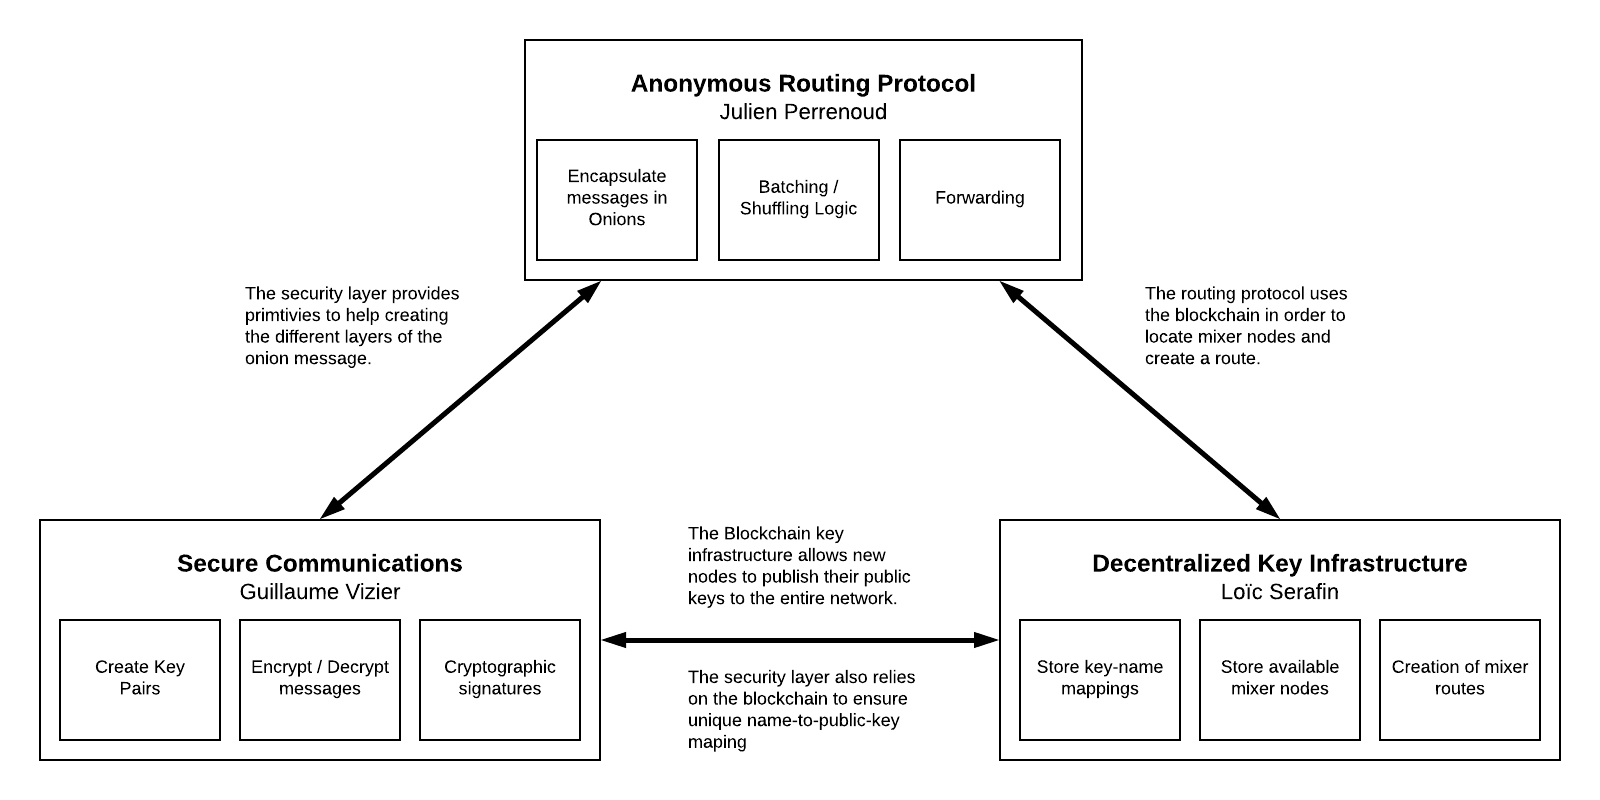
\includegraphics[width=\linewidth]{DSE Diagram.png}
  \caption{Interaction between the three sub-components}
  \label{fig:taskdiagram}
\end{figure}


\begin{thebibliography}{9}

\bibitem{chaum84}
  David L. Chaum,
  \textit{Untraceable Electronic Mail, Return Addresses, and Digital Pseudonyms},
  1984.

\bibitem{mixminion}
  George Danezis, Roger Dingledine, Nick Mathewson,
  \textit{Mixminion: Design of a Type III Anonymous Remailer Protocol},
  2002.

\bibitem{tor}
    Roger Dingledine, Nick Mathewson, Paul Syverson,
    \textit{Tor: The Second-Generation Onion Router},
    2002

\end{thebibliography}

\end{document}
